\chapter{Results}
\label{apx:results}

This appendix contains the results for experiments of identification using SSFGMM and verification using SSGMM and SSAGMM, due to the extensive number of tables and figures. Each experiment has its results shown in a separate section.

\section{Identification using SSFGMM}
\label{sec:results-identify-ssfgmm}

The identification using SSFGMM was performed for values 0.95, 0.99, 1, 1.01 and 1.05 of $r$. Similar to SSGMM, each value of $r$ is described by three tables and one figure.

\subsection{$r = 0.95$}

\begin{table}[h]
    \centering
    \begin{tabular}{|c|c|M{2cm}|M{2cm}|M{2cm}|M{2cm}|}
    \hline
    $\boldsymbol{\Delta}$ & \bf{M} & \bf{Office} & \bf{Hallway} & \bf{Intersection} & \bf{All} \\
    \hline
    \hline
     & \bf{8} & 38.70 & 44.41 & 32.37 & 50.50 \\
    \cline{2-6}
     & \bf{16} & 41.63 & 46.37 & 32.56 & 62.35 \\
    \cline{2-6}
    \multirow{5}{*}\bf{\textbf 0} & \bf{32} & 47.72 & 48.53 & 37.46 & 68.06 \\
    \cline{2-6}
     & \bf{64} & 43.75 & 50.31 & 37.27 & 72.80 \\
    \cline{2-6}
     & \bf{128} & 38.62 & 42.75 & 31.06 & 72.15 \\
    \hline
    \hline
     & \bf{8} & 33.37 & 31.67 & 26.35 & 44.87 \\
    \cline{2-6}
     & \bf{16} & 41.13 & 42.32 & 26.62 & 54.71 \\
    \cline{2-6}
    \multirow{5}{*}\bf{\textbf 1} & \bf{32} & 44.95 & 47.92 & 30.29 & 64.47 \\
    \cline{2-6}
     & \bf{64} & 43.13 & 43.36 & 31.64 & 70.95 \\
    \cline{2-6}
     & \bf{128} & 33.14 & 37.15 & 21.10 & 73.84 \\
    \hline
    \hline
     & \bf{8} & 32.21 & 33.49 & 26.66 & 43.02 \\
    \cline{2-6}
     & \bf{16} & 41.09 & 42.40 & 31.10 & 54.67 \\
    \cline{2-6}
    \multirow{5}{*}\bf{\textbf 2} & \bf{32} & 46.33 & 44.14 & 31.75 & 66.78 \\
    \cline{2-6}
     & \bf{64} & 40.93 & 43.60 & 33.53 & 72.72 \\
    \cline{2-6}
     & \bf{128} & 39.16 & 37.89 & 23.26 & 73.53 \\
    \hline
    \end{tabular}
    \caption{Identification rates for enrolled speakers with $r = 0.95$.}
    \label{tab:identify_speakers_0.95}
\end{table}


\newpage
\begin{figure}[ht]
    \centering
    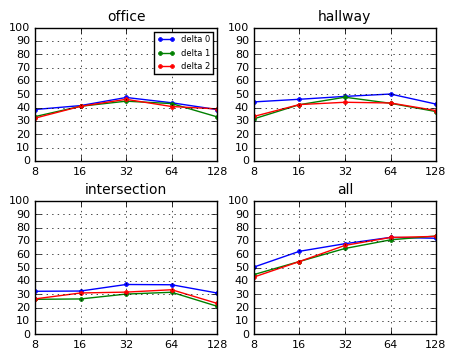
\includegraphics[width=\textwidth]{chapters/results-identify-ssfgmm/r-095}
    \caption{Identification rates for enrolled speakers using different $\Delta$s and $r = 0.95$.}
    \label{fig:r-095}
\end{figure}

\newpage
\subsection{$r = 0.99$}

\begin{table}[h]
    \centering
    \begin{tabular}{|c|c|M{2cm}|M{2cm}|M{2cm}|M{2cm}|}
    \hline
    $\boldsymbol{\Delta}$ & \bf{M} & \bf{Office} & \bf{Hallway} & \bf{Intersection} & \bf{All} \\ \hline \hline & \bf{8} & 41.55 & 51.31 & 41.13 & 63.70 \\ \cline{2-6} & \bf{16} & 47.42 & 56.13 & 45.10 & 71.64 \\ \cline{2-6}
    \multirow{5}*\bf{\textbf 0} & \bf{32} & 48.73 & 56.98 & 43.83 & 78.32 \\ \cline{2-6} & \bf{64} & 49.61 & 55.52 & 43.21 & 80.83 \\ \cline{2-6} & \bf{128} & 47.15 & 50.69 & 38.93 & 81.13 \\ \hline \hline & \bf{8} & 43.90 & 52.16 & 43.09 & 65.90 \\ \cline{2-6} & \bf{16} & 49.31 & 58.68 & 47.22 & 76.85 \\ \cline{2-6}
    \multirow{5}*\bf{\textbf 1} & \bf{32} & 52.16 & 60.42 & 48.73 & 83.37 \\ \cline{2-6} & \bf{64} & 53.94 & 60.03 & 48.77 & 86.03 \\ \cline{2-6} & \bf{128} & 49.88 & 54.63 & 45.83 & 87.15 \\ \hline \hline & \bf{8} & 43.87 & 55.25 & 43.94 & 66.63 \\ \cline{2-6} & \bf{16} & 49.65 & 60.61 & 48.11 & 77.97 \\ \cline{2-6}
    \multirow{5}*\bf{\textbf 2} & \bf{32} & 53.28 & 62.77 & 52.20 & 84.14 \\ \cline{2-6} & \bf{64} & 53.40 & 61.11 & 51.93 & 88.31 \\ \cline{2-6} & \bf{128} & 50.23 & 54.17 & 46.03 & 88.43 \\ \hline
    \end{tabular}
    \caption{Speaker identification success rates and $r = 0.99$.}
    \label{tab:identify_speakers_0.99}
\end{table}


\newpage
\begin{figure}[ht]
    \centering
    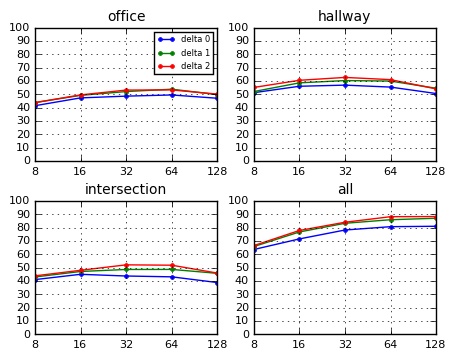
\includegraphics[width=\textwidth]{chapters/results-identify-ssfgmm/r-099}
    \caption{Identification rates for enrolled speakers using different $\Delta$s and $r = 0.99$.}
    \label{fig:r-099}
\end{figure}

\newpage
\subsection{$r = 1.00$}

\begin{table}[h]
    \centering
    \begin{tabular}{|c|c|M{2cm}|M{2cm}|M{2cm}|M{2cm}|}
    \hline
    $\boldsymbol{\Delta}$ & \bf{M} & \bf{Office} & \bf{Hallway} & \bf{Intersection} & \bf{All} \\
    \hline
    \hline
     & \bf{8} & 40.86 & 52.01 & 41.32 & 64.47 \\
    \cline{2-6}
     & \bf{16} & 47.69 & 56.52 & 44.79 & 72.22 \\
    \cline{2-6}
    \multirow{5}{*}\bf{\textbf 0} & \bf{32} & 49.50 & 57.72 & 47.61 & 77.74 \\
    \cline{2-6}
     & \bf{64} & 50.00 & 57.95 & 45.68 & 81.25 \\
    \cline{2-6}
     & \bf{128} & 48.65 & 53.43 & 42.63 & 81.67 \\
    \hline
    \hline
     & \bf{8} & 44.25 & 53.97 & 45.60 & 66.94 \\
    \cline{2-6}
     & \bf{16} & 50.42 & 62.00 & 50.54 & 78.24 \\
    \cline{2-6}
    \multirow{5}{*}\bf{\textbf 1} & \bf{32} & 54.28 & 63.54 & 53.86 & 84.45 \\
    \cline{2-6}
     & \bf{64} & 55.09 & 64.81 & 52.85 & 87.31 \\
    \cline{2-6}
     & \bf{128} & 53.32 & 59.99 & 50.46 & 88.85 \\
    \hline
    \hline
     & \bf{8} & 44.37 & 57.06 & 47.30 & 69.64 \\
    \cline{2-6}
     & \bf{16} & 50.89 & 62.81 & 52.12 & 78.78 \\
    \cline{2-6}
    \multirow{5}{*}\bf{\textbf 2} & \bf{32} & 54.90 & 65.01 & 56.29 & 86.00 \\
    \cline{2-6}
     & \bf{64} & 56.06 & 64.70 & 56.56 & 89.16 \\
    \cline{2-6}
     & \bf{128} & 52.55 & 60.73 & 49.58 & 90.66 \\
    \hline
    \end{tabular}
    \caption{Identification rates for enrolled speakers with $r = 1.00$.}
    \label{tab:identify_speakers_1.00}
\end{table}


\newpage
\begin{figure}[ht]
    \centering
    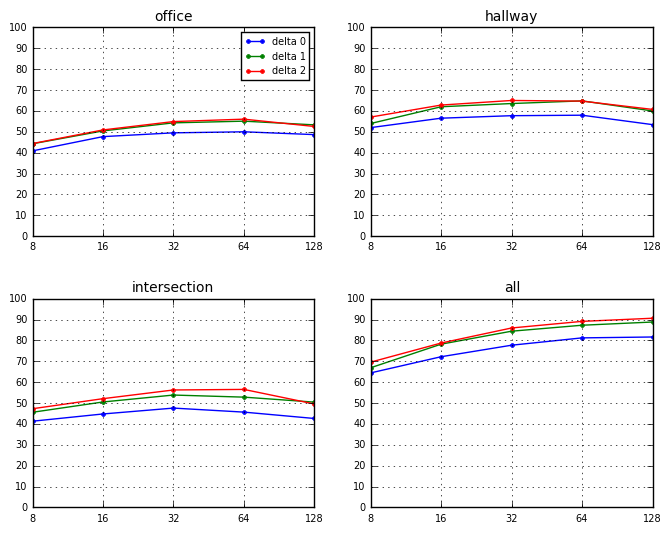
\includegraphics[width=\textwidth]{chapters/results-identify-ssfgmm/r-100}
    \caption{Identification rates for enrolled speakers using different $\Delta$s and $r = 1.00$.}
    \label{fig:r-100}
\end{figure}

\newpage
\subsection{$r = 1.01$}

\begin{table}[h]
    \centering
    \begin{tabular}{|c|c|M{2cm}|M{2cm}|M{2cm}|M{2cm}|}
    \hline
    $\boldsymbol{\Delta}$ & \bf{M} & \bf{Office} & \bf{Hallway} & \bf{Intersection} & \bf{All} \\ \hline \hline & \bf{8} & 40.16 & 52.51 & 43.02 & 61.69 \\ \cline{2-6} & \bf{16} & 46.88 & 57.10 & 47.80 & 71.84 \\ \cline{2-6}
    \multirow{5}*\bf{\textbf 0} & \bf{32} & 49.92 & 59.30 & 49.11 & 76.66 \\ \cline{2-6} & \bf{64} & 50.19 & 58.95 & 48.92 & 79.94 \\ \cline{2-6} & \bf{128} & 48.38 & 55.56 & 45.22 & 81.52 \\ \hline \hline & \bf{8} & 43.36 & 54.90 & 45.18 & 65.28 \\ \cline{2-6} & \bf{16} & 49.58 & 61.07 & 53.74 & 76.74 \\ \cline{2-6}
    \multirow{5}*\bf{\textbf 1} & \bf{32} & 55.02 & 66.44 & 56.64 & 83.60 \\ \cline{2-6} & \bf{64} & 56.02 & 66.28 & 56.25 & 88.00 \\ \cline{2-6} & \bf{128} & 55.17 & 62.23 & 54.32 & 89.51 \\ \hline \hline & \bf{8} & 45.10 & 53.74 & 47.22 & 66.44 \\ \cline{2-6} & \bf{16} & 50.81 & 64.31 & 53.59 & 78.05 \\ \cline{2-6}
    \multirow{5}*\bf{\textbf 2} & \bf{32} & 56.56 & 67.09 & 58.49 & 84.72 \\ \cline{2-6} & \bf{64} & 56.10 & 66.90 & 58.33 & 89.74 \\ \cline{2-6} & \bf{128} & 55.02 & 63.54 & 56.33 & 90.55 \\ \hline
    \end{tabular}
    \label{tab:identify_speakers_1.01}
\end{table}


\newpage
\begin{figure}[ht]
    \centering
    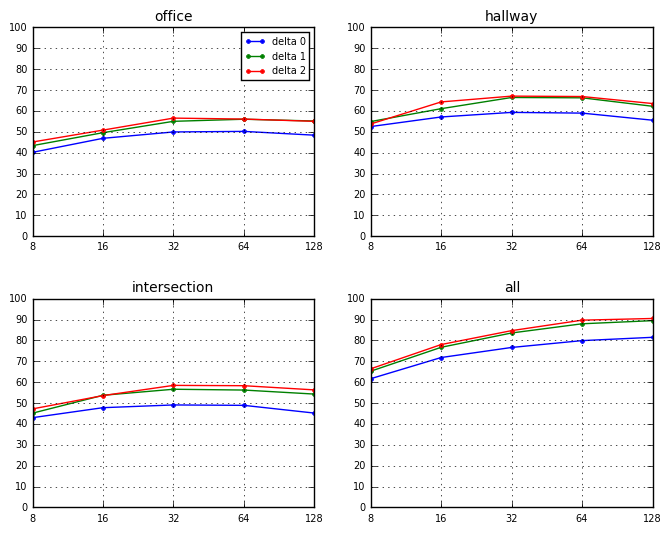
\includegraphics[width=\textwidth]{chapters/results-identify-ssfgmm/r-101}
    \caption{Identification rates for enrolled speakers using different $\Delta$s and $r = 1.01$.}
    \label{fig:r-101}
\end{figure}

\newpage
\subsection{$r = 1.05$}

\begin{table}[h]
    \centering
    \begin{tabular}{|c|c|M{2cm}|M{2cm}|M{2cm}|M{2cm}|}
    \hline
    $\boldsymbol{\Delta}$ & \bf{M} & \bf{Office} & \bf{Hallway} & \bf{Intersection} & \bf{All} \\ \hline \hline & \bf{8} & 22.22 & 33.02 & 34.80 & 30.71 \\ \cline{2-6} & \bf{16} & 32.52 & 41.32 & 42.67 & 42.32 \\ \cline{2-6}
    \multirow{5}*\bf{\textbf 0} & \bf{32} & 40.78 & 51.20 & 48.92 & 52.70 \\ \cline{2-6} & \bf{64} & 46.68 & 56.56 & 53.51 & 62.19 \\ \cline{2-6} & \bf{128} & 49.15 & 59.57 & 55.13 & 69.91 \\ \hline \hline & \bf{8} & 18.56 & 23.88 & 26.97 & 22.15 \\ \cline{2-6} & \bf{16} & 28.20 & 39.00 & 39.78 & 32.87 \\ \cline{2-6}
    \multirow{5}*\bf{\textbf 1} & \bf{32} & 38.39 & 51.58 & 50.46 & 50.08 \\ \cline{2-6} & \bf{64} & 49.11 & 63.46 & 58.33 & 62.96 \\ \cline{2-6} & \bf{128} & 57.99 & 66.32 & 59.41 & 75.96 \\ \hline \hline & \bf{8} & 17.52 & 25.15 & 28.43 & 19.41 \\ \cline{2-6} & \bf{16} & 28.94 & 38.27 & 42.44 & 34.30 \\ \cline{2-6}
    \multirow{5}*\bf{\textbf 2} & \bf{32} & 40.74 & 50.31 & 49.38 & 49.88 \\ \cline{2-6} & \bf{64} & 50.42 & 61.23 & 58.87 & 63.77 \\ \cline{2-6} & \bf{128} & 57.68 & 67.52 & 62.00 & 77.55 \\ \hline
    \end{tabular}
    \caption{Speaker identification success rates and $r = 1.05$.}
    \label{tab:identify_speakers_1.05}
\end{table}


\newpage
\begin{figure}[ht]
    \centering
    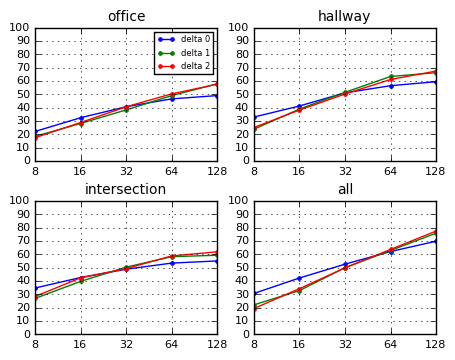
\includegraphics[width=\textwidth]{chapters/results-identify-ssfgmm/r-105}
    \caption{Identification rates for enrolled speakers using different $\Delta$s and $r = 1.05$.}
    \label{fig:r-105}
\end{figure}

\section{Verification using SSGMM}
\label{sec:results-verify-ssgmm}

\section{Verification using SSAGMM}
\label{sec:results-verify-ssagmm}

\subsection{Adapted weights}

\subsection{Adapted means}

\subsection{Adapted variances}

\subsection{Adapted weights and means}

\subsection{Adapted weights and variances}

\subsection{Adapted means and variances}

\subsection{Adapted weights, means and variances}